\documentclass[tikz,border=3pt]{standalone}
\usepackage[utf8]{inputenc}
\usepackage[T1]{fontenc}
\usepackage{lmodern}
\renewcommand{\familydefault}{\sfdefault}
\usepackage{sansmath}\sansmath
\usepackage[american]{circuitikz}
\usepackage{pgfplots}\pgfplotsset{compat=1.18,/pgf/number format/use comma,/pgf/number format/1000 sep={.}}
\usetikzlibrary{arrows.meta,calc,positioning,decorations.pathmorphing,patterns}
% paleta del sitio
\definecolor{nar}{HTML}{E8680C}\definecolor{narc}{HTML}{FFB35C}\definecolor{hielo}{HTML}{FFF3E8}
\definecolor{tinta}{HTML}{1D1D1F}\definecolor{gris}{HTML}{6E6E73}\definecolor{lila}{HTML}{7C5CF0}
\definecolor{azul}{HTML}{2F6FD6}\definecolor{menta}{HTML}{17A673}\definecolor{coral}{HTML}{E8342A}
\ctikzset{bipoles/thickness=1.6,bipoles/length=1.0cm}
\begin{document}
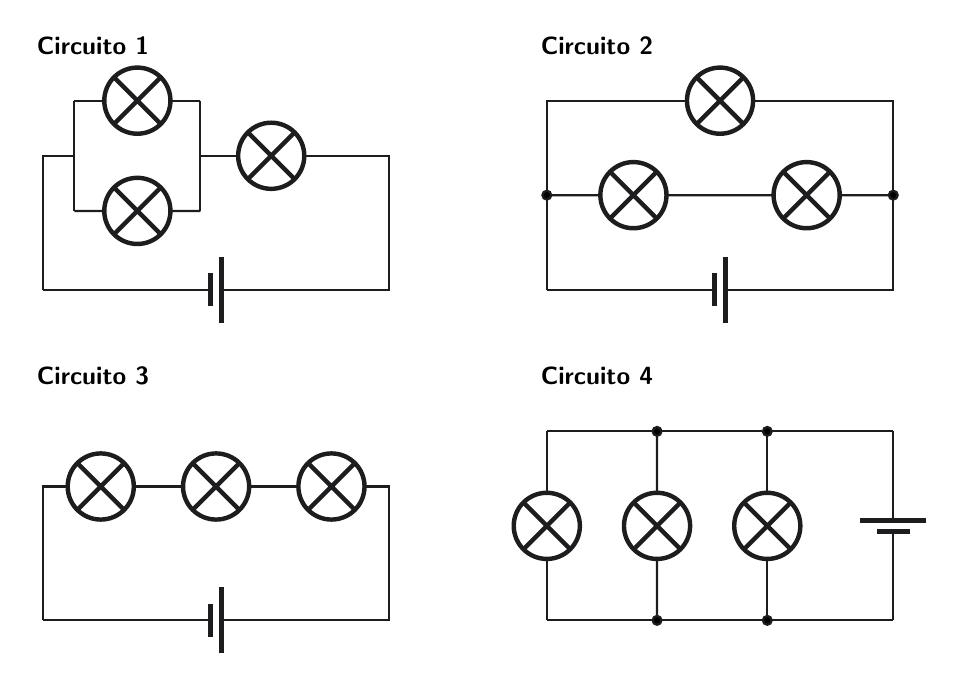
\begin{tikzpicture}[font=\small]
% circuito 1: dos en paralelo y una en serie
\begin{scope}
\node[font=\small\bfseries,anchor=west] at (-0.2,3.1) {Circuito 1};
\draw[tinta,thick] (0,0) -- (0,1.7) -- (0.4,1.7);
\draw[tinta,thick] (0.4,2.4) to[lamp] (2.0,2.4); \draw[tinta,thick] (0.4,1.0) to[lamp] (2.0,1.0);
\draw[tinta,thick] (0.4,2.4) -- (0.4,1.0); \draw[tinta,thick] (2.0,2.4) -- (2.0,1.0);
\draw[tinta,thick] (2.0,1.7) to[lamp] (3.8,1.7) -- (4.4,1.7) -- (4.4,0) to[battery1] (0,0);
\end{scope}
% circuito 2: una ampolleta en paralelo con dos en serie
\begin{scope}[xshift=6.4cm]
\node[font=\small\bfseries,anchor=west] at (-0.2,3.1) {Circuito 2};
\draw[tinta,thick] (0,0) -- (0,2.4) -- (1.4,2.4) to[lamp] (3.0,2.4) -- (4.4,2.4) -- (4.4,0) to[battery1] (0,0);
\draw[tinta,thick] (0,1.2) to[lamp,*-] (2.2,1.2) to[lamp,-*] (4.4,1.2);
\end{scope}
% circuito 3: tres en serie
\begin{scope}[yshift=-4.2cm]
\node[font=\small\bfseries,anchor=west] at (-0.2,3.1) {Circuito 3};
\draw[tinta,thick] (0,0) -- (0,1.7) to[lamp] (1.47,1.7) to[lamp] (2.93,1.7) to[lamp] (4.4,1.7) -- (4.4,0) to[battery1] (0,0);
\end{scope}
% circuito 4: tres en paralelo
\begin{scope}[xshift=6.4cm,yshift=-4.2cm]
\node[font=\small\bfseries,anchor=west] at (-0.2,3.1) {Circuito 4};
\draw[tinta,thick] (0,0) -- (4.4,0); \draw[tinta,thick] (0,2.4) -- (4.4,2.4);
\draw[tinta,thick] (0,2.4) to[lamp] (0,0);
\draw[tinta,thick] (1.4,2.4) to[lamp,*-*] (1.4,0);
\draw[tinta,thick] (2.8,2.4) to[lamp,*-*] (2.8,0);
\draw[tinta,thick] (4.4,2.4) to[battery1] (4.4,0);
\end{scope}
\end{tikzpicture}
\end{document}
